\chapter{Introduction}
\label{sec:intro}

The US offshore wind gross resource potential is over
\unit[2000]{GW}\footnote{The technical offshore wind resource potential
  that is greater than \unit[7]{m/s} annual average wind speed was
  calculated to be \unit[2058]{GW}, considering all ocean and lake areas
  less than \unit[1000]{m} depth.}, much of which is located near highly
populated coastal load centers\footnote{Excludes areas in the Great
  Lakes deeper than \unit[60]{m} because technology for floating
  structures to survive ice conditions has not been matured yet.}
\citep{resource}.  This vast potential is distributed over a resource
area of which approximately 58\% is in water that is \unit[60]{m} deep,
or greater, and that proportion rises to 95\% on the Pacific coastline
\citep{musial-ca}. The fundamental wind turbine technology shift for
deployment in deep water is the transition to buoyant support structures
from conventional fixed-bottom support structures, which become too
costly and more technically challenging in deep water (likely greater
than \unit[50]{m}) \citep{obos}. Although floating wind turbines present
many new technical challenges, they also have many potential benefits
compared to shallow-water systems.  Wind speeds can be higher in
deep-water regions because they are further from shore, although there
are exceptions to this trend.  Siting floating projects may be easier
near large load centers such as the North Atlantic, because plants
farther from shore may have fewer environmental and human use impacts,
including viewshed issues\footnote{Musial et al 2016 found that human
  use conflict diminished from 49\% inside \unit[3]{nm} to below 8\%
  outside \unit[50]{nm}}.  Despite the distance from shore, floating
systems may also be easier to install since they have the potential to
be fully assembled at regional construction ports, commissioned at
quayside, and towed out.

Preliminary analysis suggests that, in time, floating technology has the
potential to achieve a lower cost of energy than their fixed-bottom
counterparts \citep{spatial}.  In fact, the Statoil Hywind floating plant
recorded a higher capacity factor in its first few months of operation
than its fixed-bottom brethren \citep{statoil-hywind}.  However, as a
nascent technology, the cost of floating offshore wind energy is still
high today.  Detailed modeling shows that the needed long-term cost
reductions are not likely to come from a single breakthrough
invention.  Instead, significant cost reductions will come from a
disciplined combination of complementary innovations, or a technology
cost reduction \textit{pathway}.

To produce transformational cost reductions, multiple advancements are
needed over the entire system: the turbine, tower, floating platform,
moorings, anchors, construction, and logistics.  However, the
complexities of the physics, manufacturing, installation, and operation
of floating wind turbines require a fully integrated systems engineering
and techno-economic design approach to achieve these transformational
cost reductions.   The paper outlines an initial, low-fidelity
step towards realizing this vision and an example analysis.

\section{Multidisciplinary Analysis and Optimization (MDAO)}
A systems engineering framework advocates for an
\textit{integrated} approach to design, where all disciplines, costs,
performance measures, and constraints are considered concurrently.
Essentially, an analysis framework for wind plants must capture the
entire power path, from the aerodynamics to the generator and grid; the
entire load path, from the nacelle through the tower and foundation; and
the entire balance sheet, from concept through decommissioning.
Executing this proposed approach in a closed-loop optimization framework
is critical to achieve superior cost and performance gains.
A graphical depiction of this idea is shown in Figure
\ref{fig:mdao}.

\begin{figure}[htbp]
  \begin{center}
    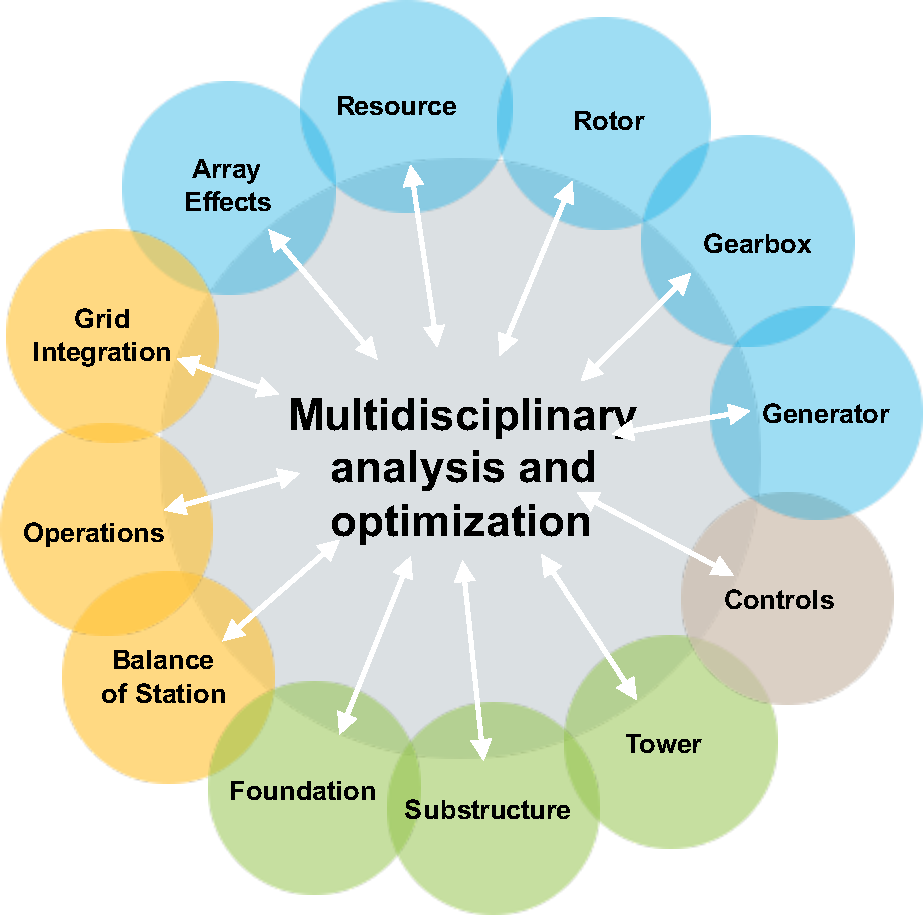
\includegraphics[width=2.5in]{mdao}
  \caption{``Integrated'' multidisciplinary design analysis and optimization
    (MDAO) approach.}
  \label{fig:mdao}
  \end{center}
\end{figure}

Multidisciplinary analysis and optimization (MDAO) would be beneficial
for all wind turbine systems, but perhaps even more so for floating
offshore systems due to their lower level of maturity, compliant nature
(motion in all six degrees of freedom), and tight inter-dependencies
among their subsystems. The stiffness and damping of the structural
members in the load path can impact the power production of the
turbine. The characteristics that minimize balance of station costs must
be integrated at the outset into the designs of the power generation and
load paths. The control systems at the turbine and plant level must
balance the demands of immediate power generation versus long-term
fatigue of the components.

MDAO has its roots in the aerospace industry with publications reaching
back into the 1960s and 1970s \citep{schmit60, haftka1977}. It grew
within aerospace and expanded to many more industries with its own
dedicated conferences and professional organizations. See
\citet{martins2013} for a more comprehensive review. With its close ties
to the aerospace industry, the wind industry was also a natural
application for MDAO practitioners. \citet{kuhn99} performed one of the
first cost-based optimizations of an offshore wind plant in 1999. Later,
\citet{dykes2011} provided a detailed review and position paper on
systems engineering and MDAO for wind energy, which triggered the
development of the Wind-Plant Integrated System Design \& Engineering
Model (WISDEM) tool. For instance, \citet{ning2014} analytically
obtained a cost of energy decrease of 5\% for land-based sites and 2\%
for offshore sites by loosening constraints on rotor tip
speed. \citet{fleming2016} showed the ability to increase the power
density of a wind farm by approximately 30\%. Concurrently,
\citet{maki2012} published one of the first system-level optimizations
of a wind turbine and found potential for a nearly 30\% decrease in the
cost of energy. \citet{ashuri2014} used MDAO principles in a system
optimization of an offshore turbine and showed a 2.3\% improvement in
levelized cost of energy (LCOE) over an NREL 5-MW reference
turbine. This work was focused on the aero-structural interactions of
the blades, rotor, and tower and had only loose coupling to wind plant
and balance-of-system (BOS) models.  \citet{bottasso2012} started
developing a research-focused systems engineering framework, with
emphasis on the rotor.  This work used multiple inner optimizations
instead of one global optimization and culminated in an excellent
summary paper by \citet{bortolotti2016}.  By most accounts, future
interest in MDAO will persist, both within the academic and industrial
wind energy community.  In fact, the number of contributors and papers
has grown so large that it was not possible to properly cite all the
interesting works in this report.

The International Energy Agency (IEA) has also recognized the need for
systems engineering tools. A research task has recently been initiated
under the IEA, Wind Task 37 – Wind Energy Systems Engineering:
Integrated Research, Design, and Development.  This task aims to
coordinate international research activities, towards the analysis of
wind power plants as holistic systems by improving the practice and
application of systems engineering to wind energy research and
development.  A couple notable publications from this effort include
\citet{perez2016}, describing a research roadmap for MDAO in wind
energy, and \citet{perez2018}, which proposed a reference offshore wind
plant, designed with MDAO.

Short of considering the entire offshore turbine, a number of authors
have focused on optimization of one or more components using MDAO
techniques. Much of this work has centered on the substructure,
including both fixed-bottom jackets/monopiles and floating substructures
(see \citep{muskulus2014}). One prominent example was the LIFES50+
consortium, which attempted to develop innovative substructure designs
to lower the LCOE of floating offshore wind plants using many MDAO
principles \citep{lifes50-framework}. LIFES50+ has examined four
candidate floating concepts and is pursuing a rigorous model and
experimental performance validation of two down-selected designs. In
addition, \citet{damiani2016} showed the application of a systems
engineering tool to optimize the cost of building a fixed-bottom jacket
structure at various locations in the United States. The optimization
itself was only focused on the mass of the structure, but the LCOE of
the optimized designs were compared, including the costs of
manufacturing and installation. Similarly, \citet{haafele2016} examined
the optimization of a jacket substructure using a cost function that
includes the raw material costs as well as contributions of
manufacturing, transport, and installation, and they found the ability
to reduce costs by over 20\%. Finally, \citet{lozano2011} used the
TOPSIS (Technique for Order Preference by Similarity to Ideal Solution)
tool to incorporate both environmental and lifetime cost considerations
to determine the most appropriate support structure for an offshore wind
site. \citet{karimi2017} used a genetic algorithm to mix and match
geometry components to create optimal hybrid substructures.  This is the
work that most closely resembles the analysis presented in this paper,
with some differences, of course.

\section{Role of Experience in MDAO for Floating Offshore Wind Energy}
One common misconception with MDAO is that the design framework and
optimization algorithms replace the engineer and dilute the value of
experience.  For the application of floating offshore wind energy
systems, this statement is far from the truth.  The hierarchy of design
criteria that sequentially narrow the design space is shown in Figure
\ref{fig:tradespace}.  First, to move to designs that will physically
survive and produce net energy, international consensus-based standards
through the International Electrotechnical Commission (IEC) and American
Petroleum Institute (API) must be met.  These standards are encapsulated
in design frameworks, such as the one proposed here, through
constraints.  Most of the floating wind prototype designs would probably
meet a basic set of certification requirements, even though
internationally recognized standards are still in development.  However,
even a fully mature certification process would serve mainly to reduce
deployment risk, not drive innovation or push the technology towards
lower-cost designs.  This is the motivation for the second step in
Figure \ref{fig:tradespace}, which arrives at a smaller region of the
tradespace that encompasses the designs with the potential to be
cost-competitive.  Concepts in this space satisfy a rubric of criteria
focused on lowering cost learned via experience.  Meaning, the
real-world lessons gained from floating turbine prototypes and tank
tests are also imbued into the design framework.  Experience manifests
itself in the underlying architecture of the design framework, its
parameterization of the geometry, the constraints, design variables, and
other options available to the user.  Without this experience, the
optimized designs that come out of the framework would likely fall to
gain credibility among the offshore wind community.  Once the tradespace
is sufficiently narrowed by standards and experience, then the
optimization is used to maximize performance This allows the engineers
and optimization tools to focus their resources on the region of the
tradespace that has the greatest cost-reduction potential.

\begin{figure}[htbp]
  \begin{center}
    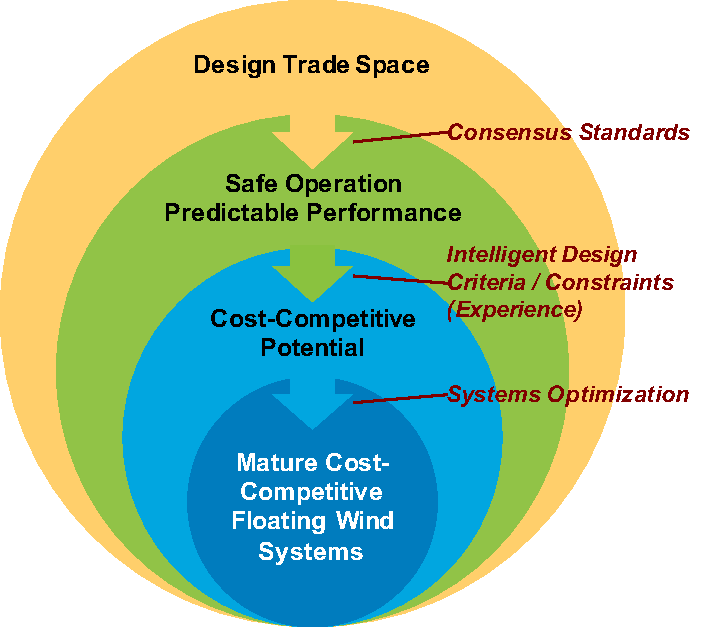
\includegraphics[width=3in]{tradespace}\\
    \caption{Narrowing the tradespace to accelerate floating system optimization.}
    \label{fig:tradespace}
  \end{center}
\end{figure}


\section{Modeling Framework}
WISDEM is selected as the platform for development of the design
framework envisioned in this paper.  The Wind-Plant Integrated System
Design and Engineering Model (WISDEM), developed by NREL, is a set of
integrated modules that creates a virtual, vertically integrated wind
plant. The models use engineering principles for conceptual design and
preliminary analysis, and link to financial modules for LCOE
estimation. The modules can be thought of as templates, in that they can
be easily tweaked for any analysis question by considering any variable
a design variable and any output an optimization objective or
constraint. The WISDEM modules are built around the OpenMDAO library \citep{openmdao},
allowing for the modules to be exercised individually for component
analysis or in unison for turbine or plant level studies.  

\begin{figure}[htbp]
  \begin{center}
    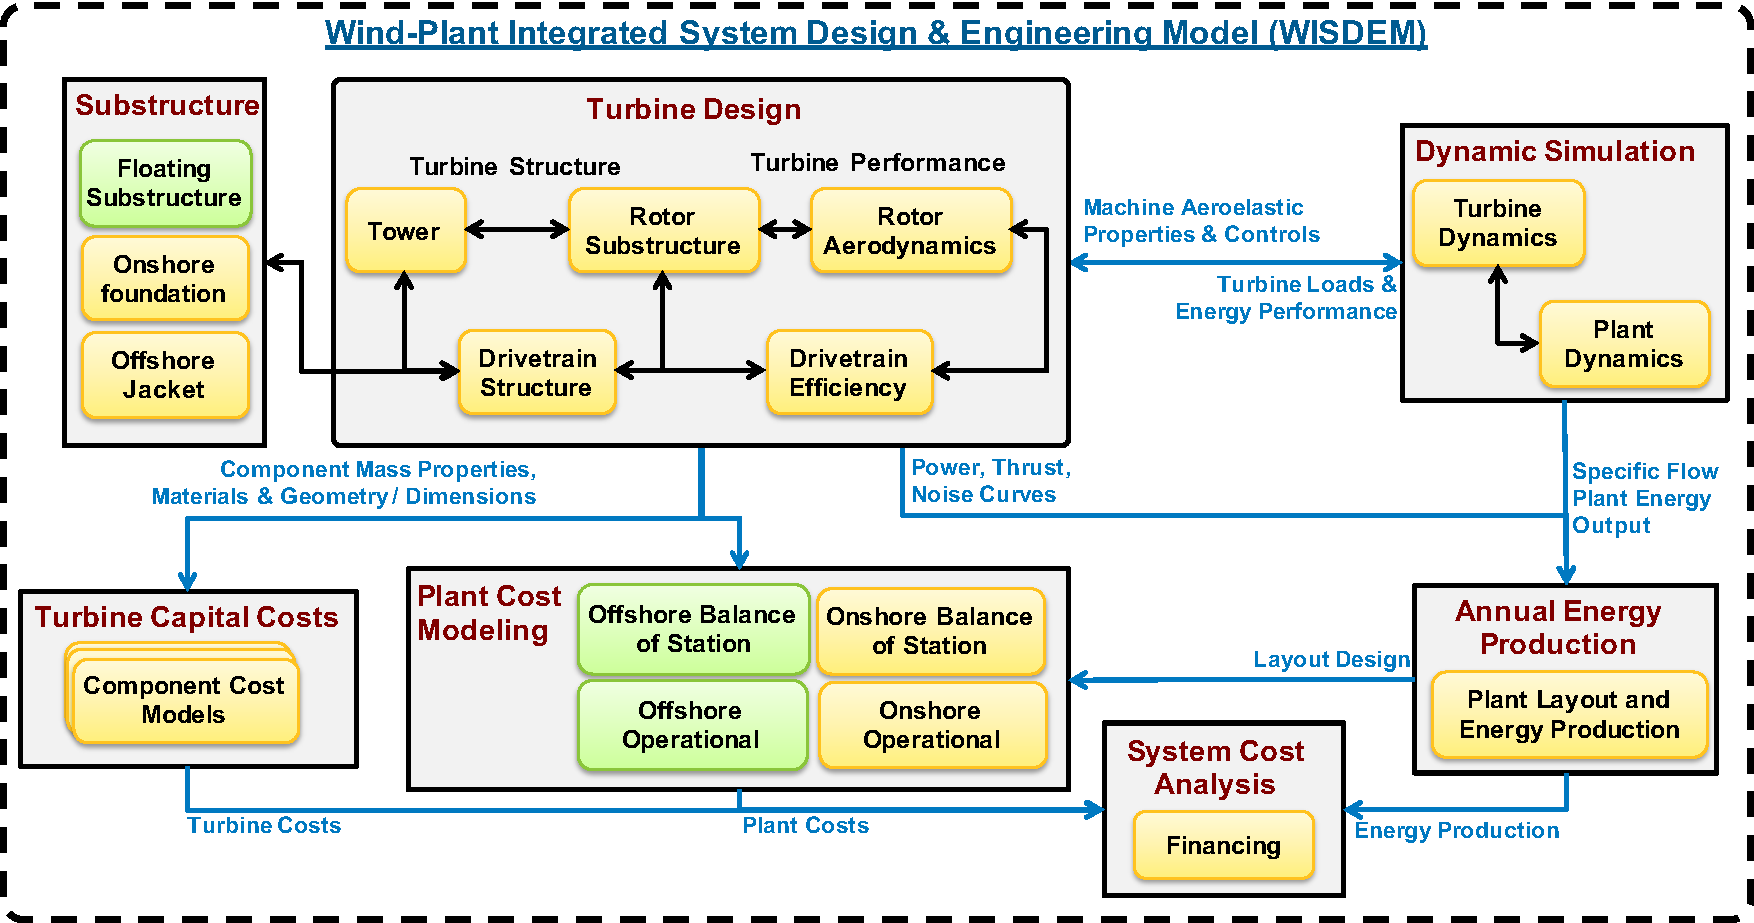
\includegraphics[width=5in]{new_wisdem}\\
    \caption{Update of WISDEM to include floating wind design modules.
      Yellow denotes an existing module and green colored modules are
      those that will be developed in this effort (note that
      fixed-bottom offshore turbines and support structures are already
      modeled).}
    \label{fig:wisdem}
  \end{center}
\end{figure}

WISDEM and the OpenMDAO library provide a solid platform from which to
develop the necessary tools for a system-level optimization methodology
for floating wind systems.  A diagram of WISDEM, with highlights of the
new modules added in course of this project is shown in Figure
\ref{fig:wisdem}.  WISDEM accounts for most of the turbine disciplines
and components involved, except most notably the floating substructures.
At the plant level, the balance of station economics for floating wind
systems from concept through decommissioning was incorporated in WISDEM
from other another in-house NREL model.  No current open-source offshore
operations and maintenance module suitable for use in WISDEM is
currently available, but development of one is part of future plans.

The key addition to WISDEM to enable floating offshore wind energy
systems to be included in its framework is the creation of the
\textit{FloatingSE} module.  This module handles conceptual cost and
sizing design of floating substructures by parameterizing the geometry
and analyzing candidate configurations with low-fidelity approximations
of loads, stress analysis, mooring system behavior, stability criterion,
and compliance with existing codes and standards.  A flow chart of the
key analysis steps and tools is shown in Figure \ref{fig:floatingse}.
\textit{FloatingSE} is made available to the broader community via
GitHub as an open-source mode.

\begin{figure}[htbp]
  \begin{center}
    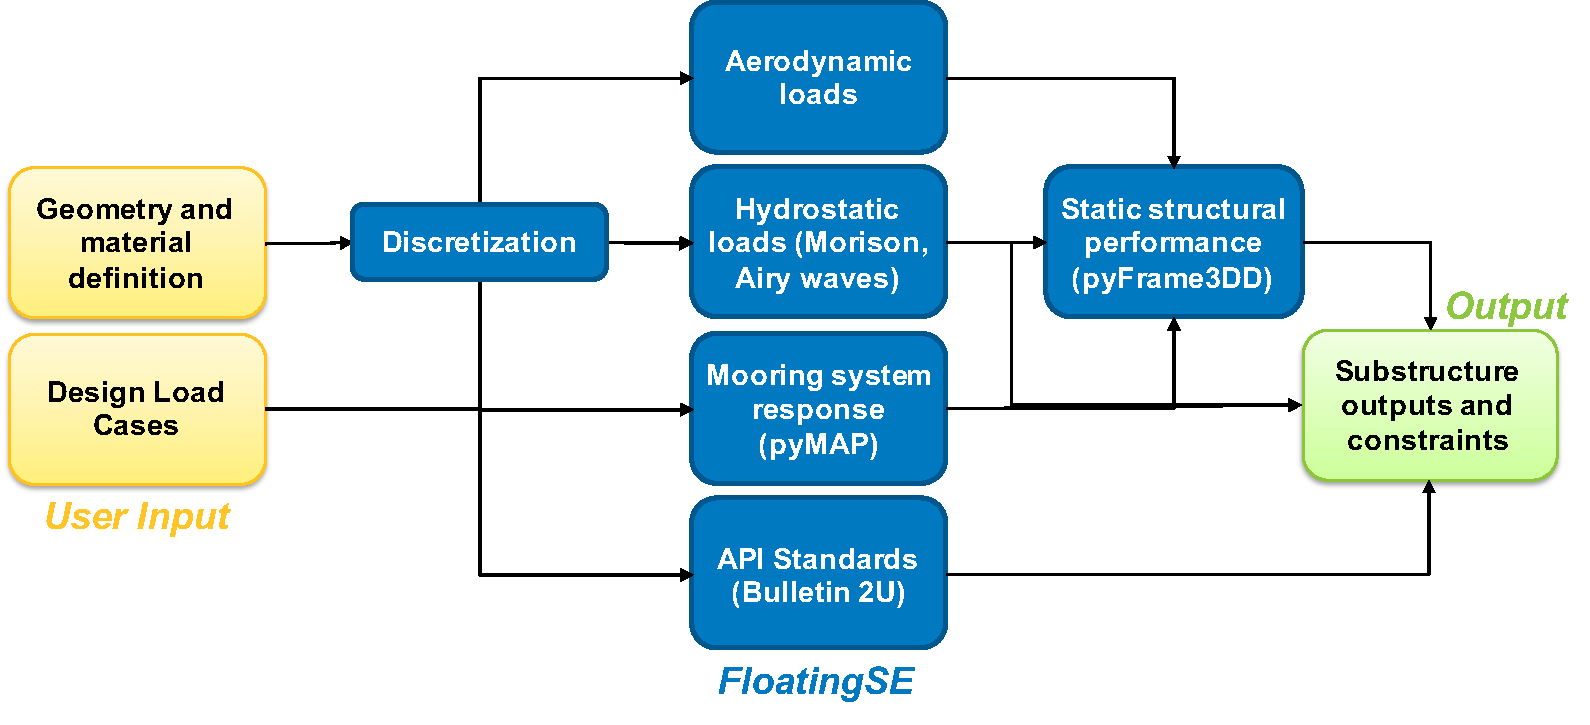
\includegraphics[width=4.5in]{floatingse}\\
    \caption{Analysis steps and tools in \textit{FloatingSE}, the floating substructure design module within WISDEM.}
    \label{fig:floatingse}
  \end{center}
\end{figure}

The next two sections of the paper present the details of
\textit{FloatingSE}.  Section \ref{sec:geom} describes the geometry
parameterization in a general manner to enable conceptual design
exploration of both classical and novel configurations.  Section
\ref{sec:theory} then describes how a design configuration is evaluated
in \textit{FloatingSE}, through the analysis flow shown in Figure
\ref{fig:floatingse}.

\section{Analysis Overview}
The final two sections of the paper feature an optimization-based design
and sensivitiy study meant to showcase the capabilities of
\textit{FloatingSE} within the WISDEM framework.  The application
features the conceptual design of three classical floating substructures
with \textit{FloatingSE}, guided only by design variable bounds and
constraints.  After showcasing the designs, a sensitivity study is
conducted where the mass of the nacelle is parameterically changed, and
the substructure designs re-optimized.  The optimization problem
formulation and solution methodology for the design and sensitivity
studies is described in Section \ref{sec:opt}.  The results of the
studies, both the conceptual designs of floating turbine substructures
and the sensitivity study, is presented in Section \ref{sec:results}.

The analysis presented here helps to quantify
the value of weight reduction in floating offshore wind turbines.
Weight minimization, and a cost premium, is a classic cost-benefit
tradeoff study that is especially germane to floating offshore wind
energy systems.  Parameterically changing the weight of the nacelle is a
surrogate for new drivetrain and generator technologies or innovations
that offer to reduce the weight of these components at a cost premium.
Without a full systems framework, it is difficult for the engineer to
make such a tradeoff.  Thus, the study here teases some of the types of
questions that could be posed and answered with the WISDEM framework to
address some of the open questions and challenges for floating offshore
wind energy systems.
